\documentclass[handout]{beamer}
\usepackage[utf8]{inputenc}
\usepackage[T2A]{fontenc}
\usepackage[english]{babel}
\usepackage{graphicx}
\usepackage{array}
\usetheme{Warsaw}
\usecolortheme{wolverine}

\usepackage{listings}
\usepackage{color}
\usepackage{amsmath}
\usepackage{changepage}

\definecolor{dkgreen}{rgb}{0,0.6,0}
\definecolor{gray}{rgb}{0.5,0.5,0.5}
\definecolor{mauve}{rgb}{0.58,0,0.82}

\lstdefinelanguage{Haskell}%
  {otherkeywords={},%
   morekeywords={as,abstype,if,then,else,case,class,data,default,deriving,%
      hiding,if,in,infix,infixl,infixr,import,instance,let,module,%
      newtype,of,qualified,type,where,do,AbsoluteSeek,AppendMode,%
      Array,BlockBuffering,Bool,BufferMode,Char,Complex,Double,Either,%
      FilePath,Float,Int,Word,Integer,Natural,IO,IOError,Ix,LineBuffering,Maybe,%
      Ordering,NoBuffering,ReadMode,ReadWriteMode,ReadS,RelativeSeek,%
      SeekFromEnd,SeekMode,ShowS,StdGen,String,Void,Bounded,Enum,Eq,%
      Eval,ExitCode,exitFailure,exitSuccess,Floating,Fractional,%
      Functor,Handle,HandlePosn,IOMode,Integral,List,Monad,MonadPlus,%
      MonadZero,Num,Numeric,Ord,Random,RandomGen,Ratio,Rational,Read,%
      Real,RealFloat,RealFrac,Show,System,Prelude,EQ,False,GT,Just,%
      Left,LT,Nothing,Right,WriteMode,True,abs,accum,accumArray,%
      accumulate,acos,acosh,all,and,any,ap,appendFile,applyM,%
      approxRational,array,asTypeOf,asin,asinh,assocs,atan,atan2,atanh,%
      bounds,bracket,bracket_,break,catch,catMaybes,ceiling,chr,cis,%
      compare,concat,concatMap,conjugate,const,cos,cosh,curry,cycle,%
      decodeFloat,delete,deleteBy,deleteFirstsBy,denominator,%
      digitToInt,div,divMod,drop,dropWhile,either,elem,elems,elemIndex,%
      elemIndices,encodeFloat,enumFrom,enumFromThen,enumFromThenTo,%
      enumFromTo,error,even,exitFailure,exitWith,fail,%
      filter,filterM,find,findIndex,findIndices,flip,floatDigits,%
      floatRadix,floatRange,floatToDigits,floor,foldl,foldM,foldl1,%
      foldr,foldr1,fromDouble,fromEnum,fromInt,fromInteger,%
      toInteger,fromJust,fromMaybe,fromRat,fromRational,%
      fromRealFrac,fst,gcd,genericLength,genericTake,genericDrop,%
      genericSplitAt,genericIndex,genericReplicate,getArgs,getChar,%
      getContents,getEnv,getLine,getProgName,getStdGen,getStdRandom,%
      group,groupBy,guard,hClose,hFileSize,hFlush,hGetBuffering,%
      hGetChar,hGetContents,hGetLine,hGetPosn,hIsClosed,hIsEOF,hIsOpen,%
      hIsReadable,hIsSeekable,hIsWritable,hLookAhead,hPutChar,hPutStr,%
      hPutStrLn,hPrint,hReady,hSeek,hSetBuffering,hSetPosn,head,%
      hugsIsEOF,hugsHIsEOF,hugsIsSearchErr,hugsIsNameErr,%
      hugsIsWriteErr,id,ioError,imagPart,indices,init,inits,%
      inRange,insert,insertBy,interact,intersect,intersectBy,%
      intersperse,intToDigit,ioeGetErrorString,ioeGetFileName,%
      ioeGetHandle,isAlreadyExistsError,isAlreadyInUseError,isAlpha,%
      isAlphaNum,isAscii,isControl,isDenormalized,isDoesNotExistError,%
      isDigit,isEOF,isEOFError,isFullError,isHexDigit,isIEEE,%
      isIllegalOperation,isInfinite,isJust,isLower,isNaN,%
      isNegativeZero,isNothing,isOctDigit,isPermissionError,isPrefixOf,%
      isPrint,isSpace,isSuffixOf,isUpper,isUserError,iterate,ixmap,%
      join,last,lcm,length,lex,lexDigits,lexLitChar,liftM,liftM2,%
      liftM3,liftM4,liftM5,lines,listArray,listToMaybe,log,logBase,%
      lookup,magnitude,makePolar,map,mapAccumL,mapAccumR,mapAndUnzipM,%
      mapM,mapM_,mapMaybe,max,maxBound,maximum,maximumBy,maybe,%
      maybeToList,min,minBound,minimum,minimumBy,mkPolar,mkStdGen,%
      mplus,mod,msum,mzero,negate,next,newStdGen,not,notElem,nub,nubBy,%
      null,numerator,odd,openFile,or,ord,otherwise,partition,phase,pi,%
      polar,pred,print,product,properFraction,putChar,putStr,putStrLn,%
      quot,quotRem,random,randomIO,randomR,randomRIO,randomRs,randoms,%
      rangeSize,read,readDec,readFile,readFloat,readHex,readInt,readIO,%
      readList,readLitChar,readLn,readParen,readOct,readSigned,reads,%
      readsPrec,realPart,realToFrac,recip,rem,repeat,replicate,return,%
      reverse,round,scaleFloat,scanl,scanl1,scanr,scanr1,seq,sequence,%
      sequence_,setStdGen,show,showChar,showEFloat,showFFloat,%
      showFloat,showGFloat,showInt,showList,showLitChar,showParen,%
      showSigned,showString,shows,showsPrec,significand,signum,sin,%
      sinh,snd,sort,sortBy,span,split,splitAt,sqrt,stderr,stdin,stdout,%
      strict,subtract,succ,sum,system,tail,tails,take,takeWhile,tan,%
      tanh,toEnum,toInt,toInteger,toLower,toRational,toUpper,transpose,%
      truncate,try,uncurry,undefined,unfoldr,union,unionBy,unless,%
      unlines,until,unwords,unzip,unzip3,unzip4,unzip5,unzip6,unzip7,%
      userError,when,words,writeFile,zero,zip,zip3,zip4,zip5,zip6,zip7,%
      zipWith,zipWithM,zipWithM_,zipWith3,zipWith4,zipWith5,zipWith6,%
      zipWith7},%
   sensitive,%
   morecomment=[l]--,%
   morecomment=[n]{\{-}{-\}},%
   morestring=[b]"%
  }[keywords,comments,strings]%

\lstset{
  language=Haskell,
  showstringspaces=false,
  columns=flexible,
  keepspaces=true,
  basicstyle={\ttfamily},
  numbers=none,
  numberstyle=\tiny\color{gray},
  keywordstyle=\color{blue},
  commentstyle=\color{dkgreen},
  stringstyle=\color{mauve}
}

\title{Number theory in Haskell}
\author[Andrew Lelechenko]{Andrew Lelechenko \\ \texttt{1@dxdy.ru}}
\date{\#kievfprog, Kiev, 18.11.2017}

\def\isqrt#1{{\tt isqrt}~#1}
\def\isqrta#1{{\tt isqrt1}~#1}
\def\isqrtb#1{{\tt isqrt2}~#1}

\begin{document}

\begin{frame}
	\titlepage
\end{frame}

\begin{frame}{Why do math not in C?}

\centerline{\em\large ``Haskell is slow, use C''.}

\begin{itemize}

\item Haskell is not slow, but C is fast.

  You cannot expect to beat hundred man years after lunch.
  Example: linear algebra in BLAS and LAPACK.

\item Haskell is maintainable, C is not.

  Typical mathematical C library (especially {\em the fastest™}) comes without documentation, has arcane interface and unclear assumptions, emits uncontrolled side effects.

\end{itemize}

\end{frame}

\begin{frame}{Why do math in Haskell?}

\begin{itemize}

\item Purely functional language, similar to mathematics.

\item Terse syntax, resembling mathematical formulas.

\item Interactive mode of evaluation.

\item Quick, but sound prototyping due to the polymorphic, but strong type system.

\end{itemize}

\end{frame}

\begin{frame}{Haskell flaws for number crunching}

\begin{itemize}

\item No manual memory management.

  Chris Done, Fast Haskell: Competing with C at parsing XML,
  http://chrisdone.com/posts/fast-haskell-c-parsing-xml

\item No automatic vectorisation (SSE/AVX instructions).

  Use FFI.

  https://github.com/sergv/nn

\end{itemize}

\end{frame}

\begin{frame}{arithmoi: doing number theory in Haskell}

Initially designed to cover Project Euler (https://projecteuler.net).
Inspired by leading PARI/GP library.

\begin{itemize}
\item Modular computations.
\item Effective prime crunching algorithms.
\item Toolbox of arithmetic functions.
\item Gaussian integers.
\item Recurrent relations.
\item Riemann zeta function.
\item Integer roots and logarithms.
\end{itemize}

\end{frame}

\begin{frame}{Integer sqrt}
\begin{adjustwidth}{-1.5em}{-1.5em}

Implement {\tt isqrt} :: Integer $\to$ Integer such that

$$(\isqrt n)^2 \le n < (1 + \isqrt n)^2.$$

For example, $\isqrt 4 = 2$, $\isqrt 5 = 2$, $\isqrt 9 = 3$.

\bigskip

\begin{itemize}

\item $\isqrta n = {\tt floor}~({\tt sqrt}~({\tt fromInteger}~@{\tt Double}~n))$

\bigskip

  $\isqrta 3037000502^2 = 3037000501$. Precision loss!

\bigskip

\item $\isqrtb n = {\tt head}~({\tt dropWhile}~(\lambda r \to (r+1)^2 \le n)~[\isqrta n..])$

\bigskip

  $\isqrtb 2^{1024} = 2^{1024}$. Out of bounds!

\end{itemize}

\end{adjustwidth}
\end{frame}

\begin{frame}[fragile]{Integer sqrt}

Implement {\tt isqrt} :: Integer $\to$ Integer such that

$$(\isqrt n)^2 \le n < (1 + \isqrt n)^2.$$

\begin{itemize}

\item Heron algorithm:

  \begin{lstlisting}
  heron n =
    head $
      dropWhile (\r -> r > step r) $
        iterate step n
    where
      step r = (r + n `quot` r) `quot` 2
  \end{lstlisting}

  Valid, but slow.

\item Karatsuba square root: divide-and-conquer algorithm,
inspired by famous Karatsuba multiplication.
Takes $O(n^{1.585})$ time.
https://hal.inria.fr/inria-00072854/PDF/RR-3805.pdf

\end{itemize}

\end{frame}

\begin{frame}{Anatoly Karatsuba (1937-2008)}

  \begin{columns}[T]
    \begin{column}{.5\textwidth}
      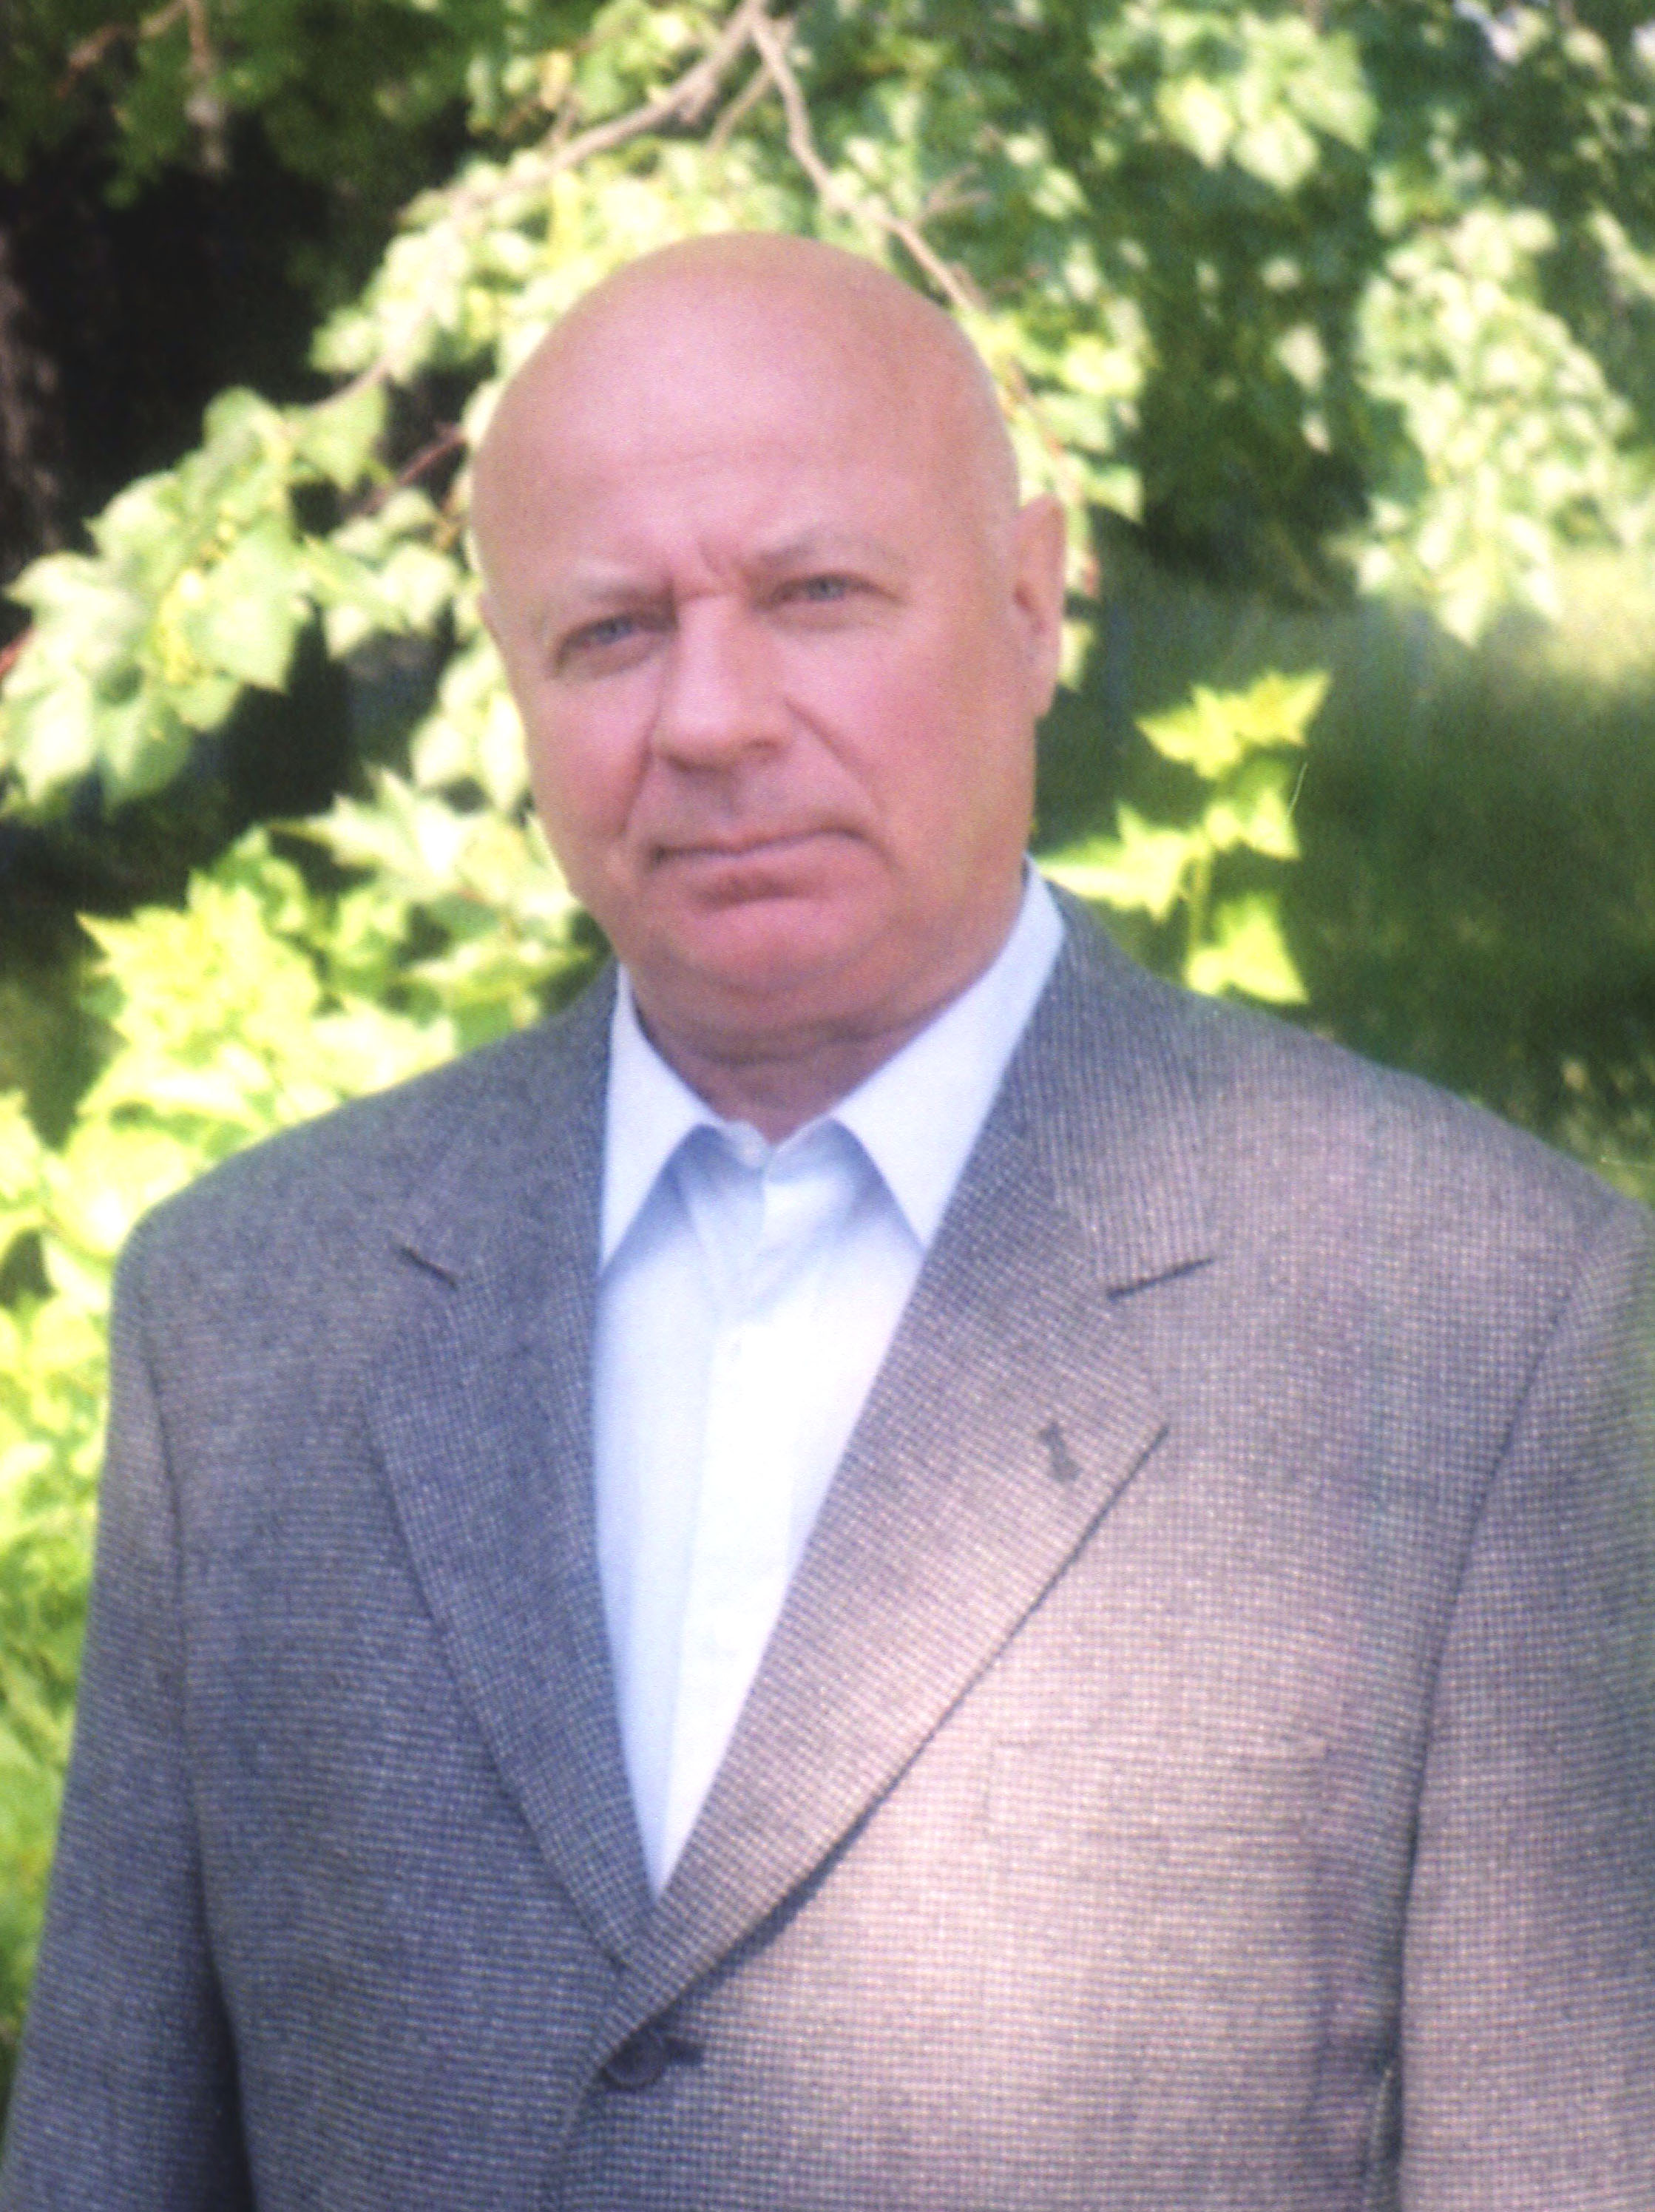
\includegraphics[width=\textwidth]{karatsuba.jpg}
    \end{column}
    \begin{column}{.5\textwidth}
        \begin{itemize}
        \item
        Research works in the field of analytic number theory,
          including trygonometric series and mean theorems.
          His results are mostly existence theorems, which do not
          provide exact constructions.

        \bigskip

        \item
        Ironically, today he is widely known
          for his fast multiplication algorithm,
          invented by accident during his study in university.
        \end{itemize}
    \end{column}
  \end{columns}

\end{frame}

\begin{frame}[fragile]{Modular power}

\begin{lstlisting}
powMod :: Integral a => a -> a -> a -> a
powMod x y m = (x ^ y) `mod` m
\end{lstlisting}

Intermediate value of $x^y$ may be extremely huge, larger than physical memory. Can we do better?

\begin{lstlisting}
powMod :: Integral a => a -> a -> a -> a
powMod x y m =
  head $
    genericDrop y $
      iterate (\n -> n * x `mod` m) 1
\end{lstlisting}

This version performs $y$ multiplications. Can we do better?

\end{frame}

\begin{frame}{Binary algorithm}

How $(\string^)$ avoids linear number of multiplications?

\begin{table}
\begin{tabular}{lllll}
& {\bf 1} & {\bf 2} & {\bf 4} & {\bf 8} \\
& $x$ & $x^2$ & $x^4$ & $x^8$ \\\hline
$11 ={}$ & 1 & 1 & 0 & 1 \\
& $x$ & $x^3$ & $x^3$ & $x^{11}$ \\\hline
$13 ={}$ & 1 & 0 & 1 & 1 \\
& $x$ & $x$ & $x^5$ & $x^{13}$
\end{tabular}
\end{table}

\end{frame}

\begin{frame}[fragile]{Binary algorithm}

\begin{lstlisting}
(^) :: Integral a => a -> a -> a
x ^ y = f x y 1

f :: Integral a => a -> a -> a -> a
f x 0 z = 1
f x 1 z = x * z
f x y z
  | even y    = f (x * x) (y `quot` 2) z
  | otherwise = f (x * x) ((y - 1) `quot` 2) (x * z)
\end{lstlisting}

Example:
$13 = 1101_2$.

$$
x^{13} = {\tt f}~x^1~13~1 = {\tt f}~x^2~6~x = {\tt f}~x^4~3~x
      = {\tt f}~x^8~1~x^5 = x^{13}
$$

Let us steal the trick!

\end{frame}

\begin{frame}[fragile]{Polymorphic powMod}

Append {\tt mod} after every multiplication:

\begin{lstlisting}
powMod :: Integral a => a -> a -> a -> a
powMod x y m = f x y 1
  where
    f :: Integral a => a -> a -> a -> a
    f x 0 z = 1
    f x 1 z = x * z `mod` m
    f x y z = f (x * x `mod` m) (y `quot` 2)
      (if odd y then (x * z `mod` m) else z)
\end{lstlisting}

\end{frame}

\begin{frame}{Boxed and unboxed}

\begin{itemize}

\item Unboxed type contains a primitive value. For instance, {\tt Word\#} is a machine-sized word, similar to its C counterpart.
\item Boxed type contains:
  \begin{itemize}
  \item Link to unboxed value.
  \item Error message.
  \item Unevaluated thunk.
  \item Blackhole.
  \end{itemize}
\item Unboxed type is always monomorphic.
\item Boxed type can be polymorphic.

\end{itemize}

\end{frame}

\begin{frame}[fragile]{Unboxed power}

Can we write more efficient implementations for concrete types?

\begin{lstlisting}
powModWord :: Word -> Word -> Word -> Word
powModWord (W# x) (W# y) (W# m) = W# (f x y 1##) where
  f :: Word# -> Word# -> Word# -> Word#
  f x 0## z = 1##
  f x 1## z = timesMod x z m
  f x y   z = f (timesMod x x m) (y `uncheckedShiftRL#` 1#)
    (if odd# y then (timesMod x z m) else z)

timesMod :: Word# -> Word# -> Word# -> Word#
timesMod x y m = r where
  (# hi, lo #) = timesWord2# x y
  (#  q, r  #) = quotRemWord2# hi lo m

odd# :: Word# -> Bool
odd# w = isTrue# (word2Int# (w `and#` 1##))
\end{lstlisting}

\end{frame}

\begin{frame}[fragile]{One interface to rule them all}

Specialize {\tt powMod} for common use cases.

\begin{lstlisting}
{-# RULES
  "powMod/Integer" powMod = powModInteger
  "powMod/Natural" powMod = powModNatural
  "powMod/Int"     powMod = powModInt
  "powMod/Word"    powMod = powModWord
  #-}
\end{lstlisting}

Mark {\tt powMod} inlinable:

\begin{lstlisting}
{-# INLINABLE powMod #-}
\end{lstlisting}

\end{frame}

\begin{frame}
\centerline{\Huge\bf Thank you!}
\bigskip
\centerline{\huge\bf github.com/Bodigrim/arithmoi}
\end{frame}

\end{document}
